\chapter{Primal Formulation: Non-Linear Model}\label{chap: deep}

In Chapter~\ref{chap: framework} we introduced a general framework for binary classification at the top samples and showed multiple formulations that fall into it. All these formulations are summarized in Table~\ref{tab: summary formulations}. In Chapter~\ref{chap: linear}, we discussed the theoretical properties of all formulations for the special case of a linear model. Since many real-world problems are not linearly separable, in Chpater~\ref{chap: dual}, we derived dual forms of all formulations and employed non-linear kernels. Moreover, we derived an efficient algorithm to solve these dual formulations. However, it is still computationally expensive.  Especially the evaluation of new samples is costly since the classification score for every new sample is computed from all training samples. More precisely, the classification score is calculated only from training samples whose corresponding dual variables are non-zero. Therefore, the dual formulations are unsuitable for large data. To overcome this issue, the following chapter is dedicated to our framework~\eqref{eq: aatp surrogate} with an arbitrary model model~$f.$ We can mention neural networks as a prototypical example of such a model. We will not discuss \Grill and \GrillNP formulations from Table~\ref{tab: summary formulations}, since their authors introduced in~\cite{grill2016learning} an algorithm to solve this formulation that is suitable even for non-linear models. Therefore, we focus only on the remaining formulations that use surrogate false-negative rate as an objective function, i.e., we assume the following general formulation
\begin{mini}{\bm{w}, \, t}{
  \frac{1}{2} \norm{\bm{w}}^2 + \frac{1}{\npos} \sum_{i \in \Ipos} l \Brac{t(\bm{w}) - f(\bm{x}_i; \bm{w})}
  }{\label{eq: aatp deep general}}{}
  \addConstraint{s_i}{= f(\bm{x}_i; \bm{w}), \quad i \in \I}
  \addConstraint{t}{= G\Brac{\bm{s}, \bm{y}},}
\end{mini}
where~$f$ is an arbitrary model. Our goal is to show how to solve this formulation in a suitable way for large data. The standard approach is to use stochastic gradient descent. To do so, we need to know the gradient of the objective function, and therefore, we assume that the model~$f$ is differentiable. The optimization problem~\eqref{eq: aatp deep general} depends on two decision variables~$\bm{w}$ and~$t.$ However, for all formulations from Table~\ref{tab: summary formulations} and each~$\bm{w}$, the threshold~$t$ can be computed uniquely. We stress this dependence by writing~$t(\bm{w})$ instead of~$t$. By doing so, we effectively remove the threshold~$t$ from the decision variables and~$\bm{w}$ remains the only decision variable. Denoting the objective of~\eqref{eq: aatp deep general} by~$L(\bm{w}),$ the chain rule implies that the gradient is equal to
\begin{equation}\label{eq: deep L gradient true}
  \nabla L(\bm{w})
    = \bm{w} + \frac{1}{\npos} \sum_{i \in \Ipos} l'\Brac{t(\bm{w}) - f(\bm{x}_i; \bm{w})}\Brac{\nabla t(\bm{w}) - \nabla f(\bm{x}_i; \bm{w})}.
\end{equation}
The only remaining part is the computation of~$\nabla t(\bm{w})$. It is simple for most of the formulations from Table~\ref{tab: summary formulations}. Moreover, Theorem~\ref{thm: differentiability} shows the computation for \PatMat.

The basic idea of the stochastic gradient descent is to split the dataset into several small minibatches~$\Imb^1, \, \Imb^2, \ldots, \, \Imb^m$ and at each iteration perform all operations only on one of them. This approach is easily applicable when for example, cross-entropy is used as an objective function since cross-entropy is additive and easily decomposable. However, in our case, the decision threshold~$t$ depends on all scores~$\bm{s},$ and consequently, the objective function is non-additive and non-decomposable. Therefore, we cannot compute the true threshold only from one minibatch, and we need to use some approximation~$\hat{t}$ of it. The most straightforward way to approximate the true threshold is to use the same rule as for the whole dataset and compute the sampled threshold~$\hat{t}$ only on data from one minibatch. By replacing all computations on the whole dataset~$\I$ with their counterparts computed only on the minibatch~$\Imb,$ we get the sampled gradient in the following form
\begin{equation}\label{eq: deep L gradient sampled}
  \nabla \hat{L}(\bm{w})
    = \bm{w} + \frac{1}{\nmbpos} \sum_{i \in \Imbpos} l'\Brac{\hat{t}(\bm{w}) - f(\bm{x}_i; \bm{w})}\Brac{\nabla \hat{t}(\bm{w}) - \nabla f(\bm{x}_i; \bm{w})}.
\end{equation}
where~$\nmbpos$ denotes the number of positive samples in the minibatch and~$\hat{t}$ denotes the sampled version of the true threshold~$t.$ The whole procedure of stochastic gradient descent for formulations from Table~\ref{tab: summary formulations} is summarized in Algorithm~\ref{alg: deep basic}.

\begin{algorithm}
  \centering
  \begin{algorithmic}[1]
    \Require Dataset~$\mathcal{D}$, minibatches~$\Imb^1,\; \Imb^2, \ldots, \; \Imb^m$, and stepsize~$\alpha^k$
    \State Initialize weights~$\bm{w}^0,$ $k \gets 0$
    \Repeat
    \State Select a minibatch~$\Imb^k$
    \State Compute scores~$\bm{s}_{\text{mb}}$ for all~$i \in \Imb^k$ as~$s_i \gets f(\bm{x}_i; \bm{w})$ 
    \State Compute sampled thershold~$\hat{t} \gets G(\bm{s}_{\text{mb}}, \bm{y}_{\text{mb}})$
    \State Compute sampled gradient~$\nabla \hat{L}$ based on~$\Imb^k$ according to~\eqref{eq: deep L gradient sampled}
    \State Set~$\bm{w}^{k+1} \gets \bm{w}^k - \alpha^k \cdot \nabla \hat{L}$
    \State Set~$k \gets k + 1$
    \Until{stopping criterion is satisfied}
  \end{algorithmic}
  \caption{Stochastic gradient descent for solving problem~\eqref{eq: aatp deep general}.}
  \label{alg: deep basic}
\end{algorithm}

\section{Bias of Sampled Gradient}\label{sec: bias sampled gradient}

In Algorithm~\ref{alg: deep basic}, we summarized a basic form of the stochastic gradient descent algorithm that can be used for any formulation from Table~\ref{tab: summary formulations} that uses surrogate false-negative rate as an objective function. The problem with this approach is that the sampled threshold~$\hat{t}$ is computed only from data from one minibatch using the same formula as for the whole dataset. However, such a choice of sampled threshold~$\hat{t}$ underestimates the true value. This issue is especially evident for \TopPush, where the sampled maximum is always smaller or equal to the true maximum. The chances that the actual maximum is in the current minibatch are small for large data. Therefore, the sampled threshold is a biased estimate of the true threshold. Another example can be the threshold for \PatMat formulation. Consider the minibatch of size 32, a typical size used in many applications. How can we compute, for example, $(0.01)$-quantile from only 32 samples? Figure~\ref{fig:thresholds1} illustrates the bias of sampled threshold for \PatMat with~$\tau=0.01$ and minibatches of different sizes. The bias between the true and sampled threshold is large, even for medium-sized minibatches. When the backpropagation is used, the sampling error is propagated through the whole gradient, and consequently, the sampled gradient is a biased estimate of the true gradient. This brings numerical issues as discussed in~\cite{bottou2018optimization}.

\begin{figure}
  \centering
  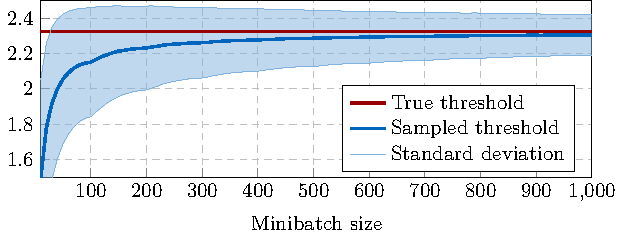
\includegraphics{images/deep_threshold_bias.pdf}
  \caption{The bias between the sampled and true thresholds computed from scores following the standard normal distribution. The threshold separates the top~$1\%$ of samples with the highest scores.}
  \label{fig:thresholds1}
\end{figure}

Convergence proofs of the stochastic gradient descent require that the sampled gradient is an unbiased estimate of the true gradient~\cite{bottou2018optimization}. In other words, the bias defined as 
\begin{equation}\label{eq:defin_bias}
  \bias(\bm{w}) := \nabla L(\bm{w}) - \EE \nabla \hat{L}(\bm{w})
\end{equation}
must equal~$0$ for all~$\bm{w}$. A comparison of~\eqref{eq: deep L gradient true} and~\eqref{eq: deep L gradient sampled} shows that a necessary condition is that the sampled threshold~$\hat{t}$ is an unbiased estimate of the true threshold~$t$. However, as we discussed above, it is not a case for Algorithm~\ref{alg: deep basic}. The following proposition quantifies the difference between the sampled and true threshold for methods that use quantile as the threshold.

\begin{proposition}[\cite{glynn1996importance}]\label{proposition:bound}
  Consider an absolutely continuous random variable~$X$ with distribution function~$F.$ Let $X_1,\, X_2, \ldots, \, X_n$ be i.i.d. samples from~$X$ and let~$\tau \in (0,1).$ Denote the true quantile~$t$ and its sampled version as~$\hat{t}$
  \begin{align*}
    t & = F^{-1}(1 - \tau), &
    \hat{t} & = F_{n}^{-1}(1 - \tau), &
  \end{align*}
  where~$F_{n}$ is the empirical distribution function. If~$F$ is differentiable with a positive gradient at~$t$, then
  \begin{equation*}
    \sqrt{n}\Brac{t - \hat{t}} \rightarrow \mathcal{N} \Brac{0, \; \frac{\tau(1-\tau)}{F'(t)^2}},
  \end{equation*}
  where the convergence is in distribution and~$\mathcal{N}$ denotes the normal distribution.
\end{proposition}

This proposition states that when the minibatch size increases to infinity, the variance of the sampled threshold is approximately
\begin{equation*}
  \frac{\tau(1-\tau)}{nF'(t)^2}.
\end{equation*}
Figure~\ref{fig:thresholds1} shows this empirically for the case where the scores follow the standard normal distribution and~$\tau=0.01$ is the desired top fraction of all samples. The approximation is poor with both significant bias and standard deviation. The natural choice to mitigate the bias is to work with large minibatches. Even though this is not a standard way, some works suggest this route~\cite{you2019large}. When the minibatch is large, it contains more samples, and the sampled threshold is more precise. However, such an approach is not applicable in many cases. For example, GPUs are often used to speed up the training process. But the usage of GPUs brings memory constraints, and therefore only small minibatches can be used in such a case.

\pagebreak

\section{\DeepTopPush}

In the previous sections, we derived Algorithm~\ref{alg: deep basic} that can be used for any formulation from Table~\ref{tab: summary formulations} that uses surrogate false-negative rate as an objective function. However, this approach provides a biased sampled gradient, and the only way to reduce the bias is to use large minibatches. In this section, we derive a new method \DeepTopPush, that mitigates this bias differently.

We start with \TopPush formulation presented in~\cite{li2014top}. Authors of~\cite{li2014top} proposed the \TopPush formulation with a linear model and solved it in its dual form. In Section~\ref{sec: ranking} we generalized this formulation for general model~$f,$ and in Chapter~\ref{chap: linear} we solved the formulation directly in its primal form for a linear model. For general model~$f,$ we stay in the primal form to be able to employ stochastic gradient descent. It means that we have the following optimization problem
\begin{mini}{\bm{w}, \, t}{
  \frac{1}{\npos} \fn(\bm{s}, t)
  }{\label{eq: toppush deep}}{}
  \addConstraint{s_i}{= f(\bm{x}_i; \bm{w}), \quad i \in \I}
  \addConstraint{t}{= \max_{j \in \Ineg} \; s_{j}.}
\end{mini}
Since the threshold always equals one of the scores~\cite{boyd2012accuracy}, its computation has a simple local formula. In other words, if the highest negative score corresponds to sample~$\bm{x}_{\indmax},$ then the gradient of the threshold equals~$\nabla t = f(\bm{x}_{\indmax}; \bm{w}).$ Therefore, the gradient of the objective function of~\eqref{eq: toppush deep} reads
\begin{equation}\label{eq: deep L gradient true toppush}
  \nabla L(\bm{w})
    = \bm{w} + \frac{1}{\npos} \sum_{i \in \Ipos} l'\Brac{f(\bm{x}_{\indmax}; \bm{w}) - f(\bm{x}_i; \bm{w})}\Brac{\nabla f(\bm{x}_{\indmax}; \bm{w}) - \nabla f(\bm{x}_i; \bm{w})},
\end{equation}
where~$\indmax$ represents the index of the negative sample with the highest score from the whole dataset. Using the same transition to the minibatches as in previous sections, we get the following formula for sampled gradient
\begin{equation}\label{eq: deep L gradient sampled toppush}
  \nabla \hat{L}(\bm{w})
    = \bm{w} + \frac{1}{\nmbpos} \sum_{i \in \Imbpos} l'\Brac{f(\bm{x}_{\indmaxmb}; \bm{w}) - f(\bm{x}_i; \bm{w})}\Brac{\nabla f(\bm{x}_{\indmaxmb}; \bm{w}) - \nabla f(\bm{x}_i; \bm{w})},
\end{equation}
where~$\indmaxmb$ represents the index of the negative sample with the highest score from the current minibatch. As discussed in the previous section, such a choice of the decision threshold provides a lower estimate of the true threshold. To improve this approximation, we modify the idea presented in~\cite{adam2019machine}. The authors of~\cite{adam2019machine} suggest using delayed classification scores to compute the threshold. We used this approach in Section~\ref{sec:convergence} to prove the convergence of stochastic gradient descent for \PatMat and \PatMatNP formulation with a linear model. However, even in such a case, the resulting sampled gradient~$\hat{t}$ is just an approximation of the true gradient~$t.$ To improve this approach, we use the fact that the threshold for \TopPush is always equal to the negative sample with  the highest score. To improve this approach, we use the fact that the threshold for \TopPush is always equal to the negative sample with the highest score. When the weights~$\bm{w}$ of model~$f$ are updated using stochastic gradient descent, the scores~$\bm{s}$ usually do not change much. It is true, especially for small learning rates. Therefore, if some negative sample has the highest score, it will likely have the highest score even after the gradient step. Since we can easily track to which negative sample this highest score corresponds, we can enhance the next minibatch by this sample. This approach significantly increases the chance that the minibatch contains the negative sample with the highest score. In such a case, the sampled threshold~$\hat{t}$ is not just an approximation but equals the true threshold~$t.$ The whole procedure is summarized in Algorithm~\ref{alg: deep toppush}.

\begin{algorithm}
  \centering
  \begin{algorithmic}[1]
    \Require Dataset~$\mathcal{D}$, minibatches~$\Imb^1,\; \Imb^2, \ldots, \; \Imb^m$, and stepsize~$\alpha^k$
    \State Initialize weights~$\bm{w}^0,$ $k \gets 0,$ and random index~$\indmaxmb$
    \Repeat
    \State Select a minibatch~$\Imb^k$
    \State Enhance minibatch~$\Imb^{\text{enh}} = \Imb^k \cup \Brac[c]{\indmaxmb}$
    \State Compute scores~$s_i \gets f(\bm{x}_i; \bm{w})$ for all~$i \in \Imb^{\text{enh}}$
    \State Find index of sampled thershold~$\indmaxmb \gets \argmax \Set{s_j}{j \in \Imb^{\text{enh}} \cap \Ineg}$
    \State Compute sampled gradient~$\nabla \hat{L}$ based on~$\Imb^{\text{enh}}$ according to~\eqref{eq: deep L gradient sampled toppush}
    \State Set~$\bm{w}^{k+1} \gets \bm{w}^k - \alpha^k \cdot \nabla \hat{L}$
    \State Set~$k \gets k + 1$
    \Until{stopping criterion is satisfied}
  \end{algorithmic}
  \caption{\DeepTopPush as an efficient method for maximizing accuracy at the top.}
  \label{alg: deep toppush}
\end{algorithm}

\begin{note}[Other formulations]\label{note: deep extension}
  Algorithm~\ref{alg: deep toppush} is applicable only on the \TopPush formulation since all other formulations use more samples to compute the threshold. However, we can modify the algorithm to be usable, for example, with \TopPushK formulation. Since \TopPushK uses the mean of~$K$ highest negative scores as a threshold, we need to enhance the current minibatch by~$K$ indices corresponding to the $K$ highest negative scores. However, since our goal was to use small minibatches, such an approach makes sense only for small~$K.$ 
\end{note}

\section{Theoretical Justification}

In the previous section, we derive \DeepTopPush method for solving the \TopPush formulation. In Section~\ref{sec: bias sampled gradient}, we discussed that the convergence proof of stochastic gradient descent requires that the sampled gradient is an unbiased estimate of the true gradient. Therefore, we are ultimately interested in the bias of the sampled gradient~$\nabla \hat{L}(\bm{w})$ defined in~\eqref{eq:defin_bias}. Recall that~$\indmax$ is the index of true threshold on the whole dataset, while~$\indmaxmb$ is the index of sampled threshold on the minibatch. We split the computation based on whether these two indices are identical or not.

\begin{restatable}{lemma}{lemmacovergencedeep}\label{lemma:convergence}
  Let~$\indmax$ be unique. Assume that the selection of positive and negative samples into the minibatch is independent and that the threshold is computed from negative samples while the objective is computed from positive samples. Then the conditional expectation of the sampled gradient satisfies
  \begin{equation*}
    \EE\Brac[s]{\nabla \hat{L}(\bm{w}) \middle\vert\indmaxmb=\indmax} =  \nabla L(\bm{w}).
  \end{equation*}
\end{restatable}

\begin{restatable}{theorem}{thmcovergencedeep}\label{theorem:convergence}
  Under the assumptions of Lemma~\ref{lemma:convergence}, the bias of the sampled gradient from \eqref{eq:defin_bias} satisfies
  \begin{equation}\label{eq:comp_bias}
    \bias(\bm{w}) = \PP\Brac[s]{\indmaxmb\neq \indmax} \Brac{\nabla L(\bm{w}) - \EE\Brac[s]{\nabla \hat{L}(\bm{w}) \middle\vert \indmaxmb\neq \indmax}}.
  \end{equation}
\end{restatable}

\pagebreak

The assumptions of Theorem~\ref{theorem:convergence} holds only for \TopPush formulation. The bias~\eqref{eq:comp_bias} consists of a multiplication of two terms. As we discussed in the previous sections, there are two strategies to reduce the bias:
\begin{enumerate}
  \item \textbf{Large minibatches:} When the minibatch is large, it contains more samples, and the chance that~$\indmaxmb$ differs from~$\indmax$ decreases. This reduces the first term in~\eqref{eq:comp_bias}. Moreover, Proposition~\ref{proposition:bound} ensures that the difference between the sampled threshold~$\hat{t}$ and the true threshold~$t$ is small. Then the difference between the true gradient~\eqref{eq: deep L gradient true toppush} and the sampled gradient~\eqref{eq: deep L gradient sampled toppush} decreases as well. This reduces the second term in~\eqref{eq:comp_bias}.
  \item \textbf{Enhanced minibatch:} The enhanced minibatch increases the chance that~$\indmaxmb$ equals~$\indmax.$ This reduces the first term in~\eqref{eq:comp_bias}. 
\end{enumerate}
The former strategy uses Algorithm~\ref{alg: deep basic} while the latter is described only for formulation~\eqref{eq: toppush deep} in Algorithm~\ref{alg: deep toppush}. For clarity, we use the name \DeepTopPush for Algorithm~\ref{alg: deep toppush} that solves formulation~\eqref{eq: toppush deep}. Similarly, we use the name \TopPush if Algorithm~\ref{alg: deep basic} is used to solve formulation~\eqref{eq: toppush deep}.

Figure~\ref{fig:thresholds2} shows the effect of the enhanced minibatch on the training. The top part of the figure compares the value of the true threshold~$t$ and its sampled version~$\hat{t}$ during training. The red dashed line represents true threshold~$t.$ The full blue line shows the sampled threshold obtained by \DeepTopPush (enhanced minibatch), while the dotted grey line the same for \TopPush. While the sampled threshold for \TopPush jumps wildly, for \DeepTopPush is smooth and often equal to the true threshold. It shows the importance of the enhanced minibatch. Moreover, Theorem~\ref{theorem:convergence} implies that for \DeepTopPush the sampled gradient is an unbiased estimate of the true gradient. It is even more pronounced in the bottom part of Figure~\ref{fig:thresholds2}, which shows the angle between the true gradient~$\nabla L$ and the sampled gradient~$\nabla \hat{L}.$ This angle is essential because~\cite{nocedal2006numerical} showed that if this angle is in the interval~$[0, 90)$, then gradient descent schemes converge. Which is precisely what happened for \DeepTopPush. When the threshold is correct, the true and sampled gradients are parallel to each other, and the gradient descent moves in the correct direction.

\begin{figure}
  \centering
  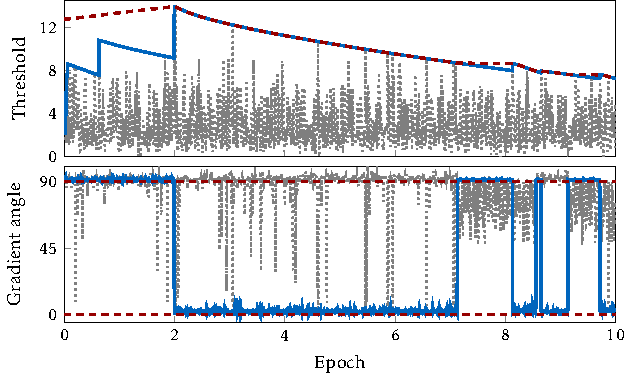
\includegraphics{images/deep_thresholds.pdf}
  \caption{The \textbf{top} figure shows the comparison of the true threshold (red dashed line) and sampled threshold for \TopPush (gray dotted line) and \DeepTopPush (blue line). The \textbf{bottom} figure shows the angle between true and sampled gradients for \TopPush (gray dotted line) and \DeepTopPush (blue line). In this case, the red dashed lines represent 0 and 90 degrees angles. The experiment was performed on the CIFAR10 dataset with a minibatch of size 32 and 10 training epochs.}
  \label{fig:thresholds2}
\end{figure}